\documentclass[tikz, margin=30mm]{standalone}
\usepackage{tikz}
\usetikzlibrary{shapes.geometric, arrows, positioning, decorations.pathreplacing, calc, matrix, fit}
\usepackage[margin=0.5cm]{geometry}


\begin{document}

\begin{tikzpicture}[node distance=2cm and 2cm,
  % every node/.style={inner sep=0,outer sep=0}
  inner/.style={draw=black!80,fill=white!20,thick, inner sep=04pt},
  outer/.style={draw=black,fill=white!10,thick,inner sep=08pt},
  mymatrix/.style={matrix of nodes, nodes=typetag, row sep=1em},
  mycontainer/.style={draw=white, inner sep=1ex},
  typetag/.style={draw=white, inner sep=1ex, anchor=west},
  title/.style={draw=none, color=white, inner sep=0pt},
  ]

  \node[outer, remember picture,outer xsep=02pt] (input) {
    \begin{tikzpicture}

      \node[] (mapper) {
        \begin{tikzpicture}
          \foreach \y in {0,1,...,8}
            {
            \node[circle, draw=black, fill=green, minimum size=0.01cm, scale=.3] at (0, -\y*0.5) {};
            \node[circle, draw=black, fill=green, minimum size=0.01cm, scale=.3] at (0.1, -\y*0.5) {};
            \node[circle, draw=black, fill=green, minimum size=0.01cm, scale=.3] at (0.2, -\y*0.5) {};
          }
        \end{tikzpicture}
      };

      \node [below=.0cm of mapper] (ssl) {Feature vectors};

      \matrix[mymatrix, below=0.1cm of ssl, draw] (mx1) {
        |[title]| \\
        % Labels \\
        Confounder Variables \\
      };
      \node[below=0.0cm of mx1, text width=4.2cm, align=center] (label3) {Annotations};


    \end{tikzpicture}
  };

\coordinate [right=4 of input] (Overfit) {};
  \node[outer, remember picture] (Overfit) at (Overfit) {
    \begin{tikzpicture}

  \node[inner, remember picture] (finetune) {
    \begin{tikzpicture}
  \node[] (monai) {
    
\includegraphics[width=1.5cm, height=1.5cm]{./MONAI-logo-color.png}
  };

      \node[below=0.0cm of monai]  (pytorch) {
    
\includegraphics[width=1.5cm, height=1.5cm]{./Pytorch_logo.png}
  };
\end{tikzpicture} };
  \node[inner, remember picture, below=0.1cm of finetune] (labelFine) { Linear Probing };

  \node[below=0.0cm of labelFine, text width=4.2cm, align=center] (UMAP) {
    \begin{tikzpicture}
      \node[] (umap) {
        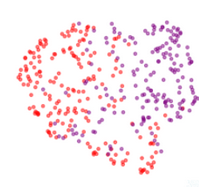
\includegraphics[width=1.5cm, height=1.5cm]{./simpleUmap.png}
      };
      \node[inner, remember picture, below=0.1cm of umap] (labelUmap) { UMAP };
    \end{tikzpicture}
    };

  \end{tikzpicture}
      };

\node[outer, remember picture, right=1.8 of Overfit] (output) {
    \begin{tikzpicture}

      \node[inner, remember picture, below=0.1cm of label3] (analysis) { LP scores };

      \node[inner, remember picture, below=0.1cm of analysis] (analysis) { UMAP plots and scores };
    \end{tikzpicture}
  };

\node [above=.0cm of input] (inputText) {Input};
\node [above=.0cm of Overfit] (overfitText) {Feature inspection plugin};
\node [above=.0cm of output] (outputText) {Output};

\draw[->] (input) -- (Overfit);
\draw[->] (Overfit) -- (output);
 
 
\end{tikzpicture}

\end{document}

